\section{Dicas Gerais}

Os slides devem apresentar uma identidade conjunta. Para isso devem ser usados estilos apropriados, que estão disponiveis nas ferramentas de criação, ou se criar um estilo novo.

Esse estilo deve possuir vários tipos de slides. A aula deve usar muitos desses tipos. Os tipos principais são:
\begin{itemize}
    \item título;
    \item o título de seção;
    \item o slide de uma coluna, o mais comum;
    \item o slide de duas colunas;
    \item o slide de duas colunas com títulos, e
    \item o slide só com título, usado para figuras.
\end{itemize}






Os slides \textbf{devem ser numerados} e conter em cada slide o número total de slides, possivelmente no formato ``slide/total'', como em ``4/40''. Eu uso número bem grandes que podem ser claramente vistos pela audiência, que assim saberá em que local está.

Todo slide deve ter um \textbf{título único}. Algumas pessoas gostam de usar um título de seção e um subtítulo que diz o que realmente o slide diz, mas isso faz com que cada slide pareça ser o mesmo que o outro e eu discordo dessa abordagem. A Figura \ref{fig:coppe} mostra um slide seguindo essa regra. A Figura \ref{fig:meio} mostra um slide que tem todas as seções identificadas em seu cabeçalho, sendo que a seção atual está com ênfase. Nesse caso, o título principal ainda é o título do slide. Isso pode ser feito automaticamente em alguns estilos para \texttt{beamer} no \LaTeX.

Todos os slides devem identificar a aula, o autor, incluindo o e-mail. Eu coloco isso no rodapé, o que é realmente o lugar para colocá-los no \textit{Power Point}. A instituição pode ser indicada através de um logo, como o slide da Figura \ref{fig:coppe}\footnote{Os slides vermelhos não têm a identificação da instituição porque são usados em mais de um curso}.

\begin{figure}[htb]
    \centering
    
\includegraphics[width=\tam\linewidth]{imagens/slideexemplotepj.png}
    \caption{Um slide com logo, um título único, identificação, número do slide e número total de slides}
    \label{fig:coppe}
\end{figure}

Use fontes ``limpas'', não rebuscadas, e \textbf{sem-serifa}\footnote{Serifas são as pontinhas que existem em algumas fontes. Elas estão bem visíveis no S da palavra ``slides'' desta seção.}, como Arial ou Calibri, e \textbf{corpos grandes}, 32 pts, por exemplo. Os slides das Figuras \ref{fig:coppe} e \ref{fig:teximag} seguem essa regra. Já o slide da figura \ref{fig:formulas} usa um tamanho menor para o corpo das fórmulas. Lembre que a banca, ao invés dos alunos, é mais velha e pode ter dificuldades de visão.

A melhor estratégia para o estilo dos slides de aula são o fundo branco, letras escuras, e cores para ressaltar. Isso se adequa bem tanto a salas bem iluminadas quanto a salas escuras, para todo tipo de projetor. A Figura \ref{fig:teximag}, apesar de usar o forte grená, me parece bastante adequada. As outras figuras  mostram outros modelos que eu uso e sinto adequados para uma aula. As cores azuis e cinzas, porém, são mais ``fracas'' e podem levar a um pouco de monotonia.

Slides ``divertidos'', como os que estão resumidos\footnote{Esses slides foram encontrados em     \url{https://unblast.com/funtastic-free-powerpoint-presentation-template-ppt/}
} na Figura \ref{fig:fun} vão criar uma carga cognitiva muito grande em uma apresentação e podem incomodar membros da banca. Já vi isso acontecer. Mas isso não quer dizer que não possam ser usados em um ou outro slide, como marcos de início de seção ou outra alternativa de menor impacto que usá-los em toda aula.

\begin{figure}[hbt]
    \centering
    
\includegraphics[width=\tam\linewidth]{imagens/funslide.jpg}
    \caption{Exemplos de slides divertidos.
        (Fonte: unblast.com) }
    \label{fig:fun}
\end{figure}


É importante variar o estilo do slide. Isso é bem fácil no \textit{Power Point}, porém é mais difícil no \texttt{beamer}, por exemplo. A Figura \ref{fig:man} mostra um slide bem diferente do que os apresentados normalmente, mas ainda em um formato ``retangular''. Use os formatos para tirar a monotonia da aula. Use também animações nos slides, mas cuidado com as transições entre os slides, que devem ser usadas muito parcimoniosamente, porque quebram a atenção.

\begin{figure}[htb]
    \centering
    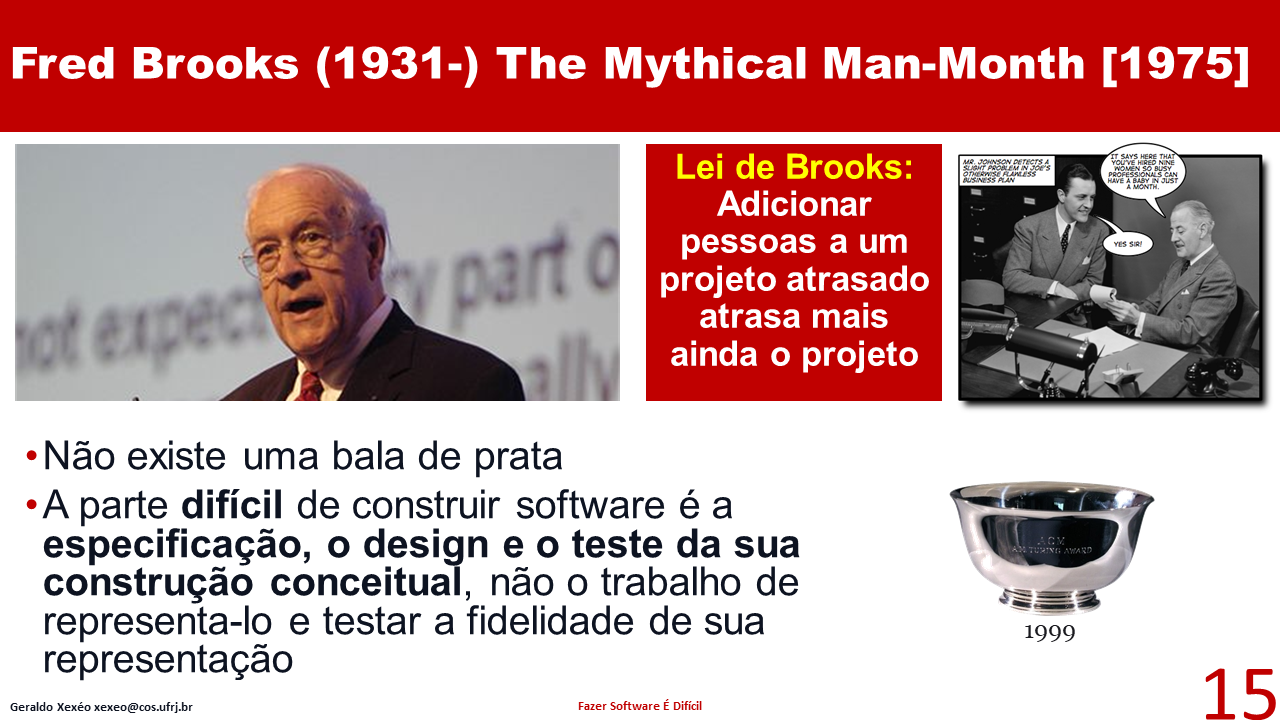
\includegraphics[width=\tam\linewidth]{imagens/manmonth.png}
    \caption{Um slide com um formato diferente}
    \label{fig:man}
\end{figure}


Os slides não devem ser exagerados, nem em texto, nem em decoração, porém um ou outro slide pode ser mais divertido, ou mais pesado em texto.

Em um slide com fórmulas, como o da Figura \ref{fig:formulas}, elas devem aparecer uma a uma se estiverem sendo calculadas. Se for apenas um comentário sobre a complexidade das fórmulas, que você deseje passar por cima em busca de uma explicação mais fácil, elas podem aparecer todas de uma vez.

\begin{figure}[hbt]
    \centering
    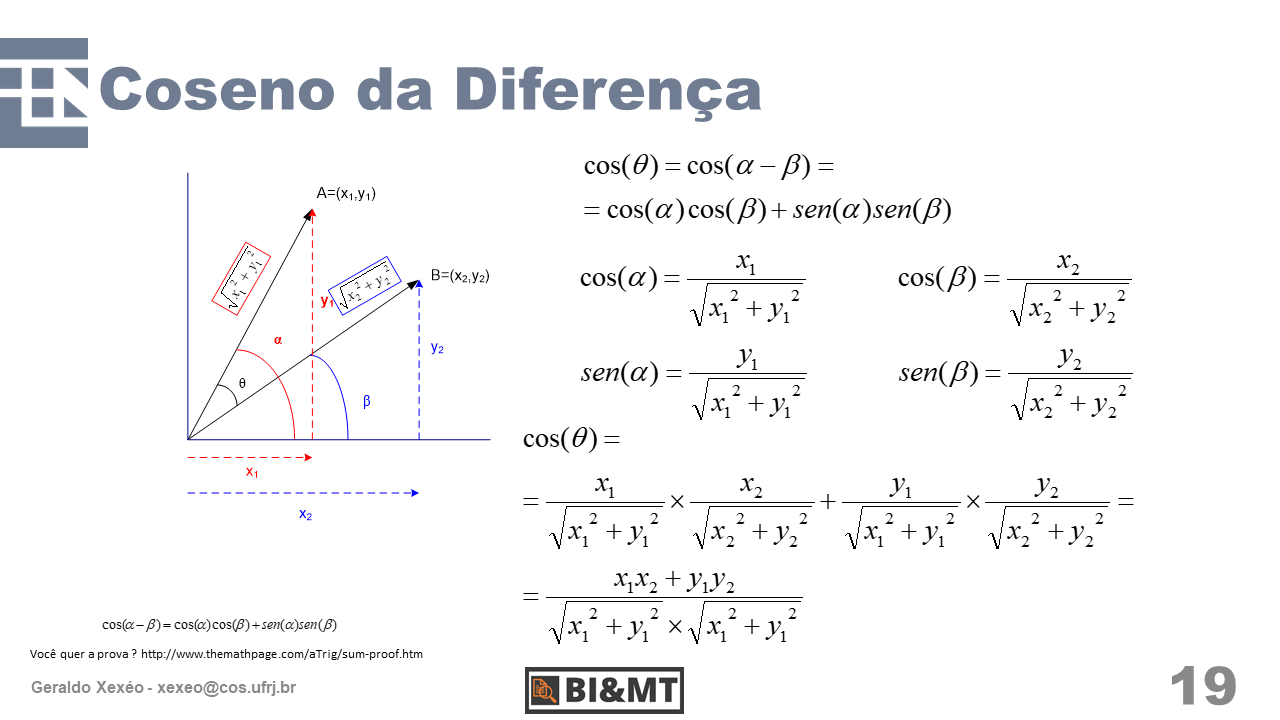
\includegraphics[width=\tam\linewidth]{imagens/desenhoeformulas.png}
    \caption{Desenho e fórmulas em um slide, que possui o logo do laboratório ligado ao curso e um logo que foi criado para identificar o curso em 3 lugares: Moodle, Whatsapp e GitHub.}
    \label{fig:formulas}
\end{figure}